\documentclass[12pt, xcolor={dvipsnames}]{beamer}
\mode<presentation>{
  \usetheme{Madrid}
  % or ...
  \usecolortheme[named=OliveGreen]{structure}
  \setbeamercovered{transparent}
  % or whatever (possibly just delete it)
}
% -- Add this section to your LaTeX doc
% Remember to use "pdflatex -shell-escape myfile.tex"
% or it won't allow LaTeX to call any command-line
% programs!
\usepackage{graphicx}

\graphicspath{{../images/}}
\newcounter{smilescounter}
\setcounter{smilescounter}{1}
\newcommand{\smiles}[1]{
\immediate\write18{obabel -:"#1" -O ../images/SMILES/smilesimg\arabic{smilescounter}.png}
\centering\includegraphics[width=0.1\textwidth]{../images/SMILES/smilesimg\arabic{smilescounter}.png}
\addtocounter{smilescounter}{1}
}
% -- End of section 
\newcommand{\Ala}{C[C@@H](N)C(=O)O }
\newcommand{\Arg}{N[C@@H](CCCNC(=N)N)C(=O)O }
\newcommand{\Asn}{N[C@@H](CC(=O)N)C(=O)O }
\newcommand{\Asp}{NC(CC(O)=O)C(O)=O}
\newcommand{\Cys}{C([C@@H](C(=O)O)N)S} %
\newcommand{\Glu}{C(CC(=O)O)C(C(=O)O)N}
\newcommand{\Gln}{O=C(N)CCC(N)C(=O)O}
\newcommand{\Gly}{C(C(=O)O)N}
\newcommand{\His}{O=C(O)[C@@H](N)Cc1cncn1}
\newcommand{\Ile}{CC[C@H](C)[C@@H](C(=O)O)N}
\newcommand{\Leu}{CC(C)C[C@@H](C(=O)O)N}
\newcommand{\Lys}{C(CCN)CC(C(=O)O)N}
\newcommand{\Met}{CSCCC(C(=O)O)N}
\newcommand{\Phe}{N[C@@H](Cc1ccccc1)C(=O)O } %fix
\newcommand{\Pro}{OC(=O)C1CCCN1}
\newcommand{\Ser}{C([C@@H](C(=O)O)N)O}
\newcommand{\Thr}{C[C@H]([C@@H](C(=O)O)N)O}
\newcommand{\Trp}{c1ccc2c(c1)c(c[nH]2)C[C@@H](C(=O)O)N}
\newcommand{\Tyr}{N[C@@H](Cc1ccc(O)cc1)C(O)=O}
\newcommand{\Val}{CC(C)[C@@H](C(=O)O)N}
\newcommand{\Sec}{O=C(O)[C@@H](N)C[SeH]}
\newcommand{\Pyl}{O=C(NCCCC[C@@H](C(=O)O)N)}


\usepackage[T2A,T1]{fontenc}
\usepackage[utf8x]{inputenc}

\usepackage[russian]{babel}

\usepackage{graphics}

\usepackage{wrapfig}
\usepackage{tikz}
\usetikzlibrary{positioning,arrows}
\usepackage{tikz}
\usepackage{xparse}

\DeclareDocumentCommand{\Lysine}{ O{red} O{0.5} m }{
	\begin{scope}[scale=#2]	% Lysine
	\path (#3) node (zero) {};
	\draw[to_2]  (zero.center)	-- ++(30:1) node (CO) {}
	        -- +(330:1) node [anchor=base] {O$^{\mbox{-}}$};
	\draw[to_1]  (CO.center) 	-- +(90:1) node (Od) {O};
	\draw[to_1i] (CO.30)		-- +(90:1);
	\draw[to_3]  (zero.center)	-- ++(150:1) node {NH$_{\mbox{3}}^{\mbox{+}}$};
	\draw[to_3, #1]  (zero.center)	-- ++(270:1) node(Cb){}
	        -- ++(330:1) node (Cc) {}
	        -- ++(270:1) node (Cd) {}
	        -- ++(210:1) node (Ce) {}
	        -- ++(150:1) node (Cf) {NH$_{\mbox{2}}$};
	\end{scope}
}

\DeclareDocumentCommand{\Asparagine}{ O{red} O{0.5} m }{
	\begin{scope}[scale=#2]	% Asparagine
	\path (#3) node (zero) {};
	\draw[to_2]  (zero.center)	-- ++(30:1) node (CO) {}
	        -- +(330:1) node [anchor=base] {O$^{\mbox{-}}$};
	\draw[to_1]  (CO.center)	-- +(90:1) node (Od) {O};
	\draw[to_1i] (CO.30)		-- +(90:1);
	\draw[to_3]  (zero.center)	-- ++(150:1) node {NH$_{\mbox{3}}^{\mbox{+}}$};
	\draw[to_2,#1]  (zero.center)	-- ++(270:1) node(Cb){}
	        -- ++(330:1) node (Cc) {}
	        -- +(30:1) node (Cd) {NH$_{\mbox{2}}$};
	\draw[to_1i,#1] (Cc.center)	-- +(270:1) node (O) {};
	\draw[to_1,#1]  (Cc.210)		-- (O.150);
	\path[#1] (O.center) node {O};
	\end{scope}
}

\DeclareDocumentCommand{\Arginine}{ O{red} O{0.5} m }{
	\begin{scope}[scale=#2]	% \Arginine
	\path (#3) node (zero) {};
	\draw[to_2]  (zero.center)	-- ++(30:1) node (CO) {}
	        -- +(330:1) node [anchor=base] {O$^{\mbox{-}}$};
	\draw[to_1]  (CO.center)	-- +(90:1) node (Od) {O};
	\draw[to_1i] (CO.30)		-- +(90:1);
	\draw[to_3]  (zero.center)	-- ++(150:1) node {NH$_{\mbox{3}}^{\mbox{+}}$};
	\draw[to_2, #1]  (zero.center)	-- ++(270:1) node(Cb){}
	        -- ++(330:1) node (Cc) {}
	        -- ++(270:1) node (Cd) {}
	        -- ++(330:1) node (NH1) {NH};
	\draw[from_2,to_3,#1]  (NH1.center)	-- ++(30:1) node (Ce) {}
	        -- ++(330:1) node {NH$_{\mbox{2}}$};
	\draw[to_1i,#1] (Ce.center)	-- ++(90:1) node (N2) {};
	\draw[to_1,#1]  (Ce.150)		-- (N2.210);
	\path[#1] (N2) node {N};
	\end{scope}
}

\DeclareDocumentCommand{\Serine}{ O{red} O{0.5} m }{
	\begin{scope}[scale=#2]	% Serine
	\path (#3) node (zero) {};
	\draw[to_2]  (zero.center)	-- ++(30:1) node (CO) {}
	        -- +(330:1) node [anchor=base] {O$^{\mbox{-}}$};
	\draw[to_1]  (CO.center)	-- +(90:1) node (Od) {O};
	\draw[to_1i] (CO.30)		-- +(90:1);
	\draw[to_3]  (zero.center)	-- ++(150:1) node {NH$_{\mbox{3}}^{\mbox{+}}$};
	\draw[to_2,#1]  (zero.center)	-- ++(270:1) node(Cb){} -- ++(210:1) node (Cc) {OH};
	\end{scope}
}
\DeclareDocumentCommand{\Threonine}{ O{red} O{0.5} m }{
	\begin{scope}[scale=#2]	% Threonine
	\path (#3) node (zero) {};
	\draw[to_2]  (zero.center)	-- ++(30:1) node (CO) {}
	        -- +(330:1) node [anchor=base] {O$^{\mbox{-}}$};
	\draw[to_1]  (CO.center)	-- +(90:1) node (Od) {O};
	\draw[to_1i] (CO.30)		-- +(90:1);
	\draw[to_3]  (zero.center)	-- ++(150:1) node {NH$_{\mbox{3}}^{\mbox{+}}$};
	\draw[to_2,#1]  (zero.center)	-- ++(270:1) node(Cb){}
	        -- ++(330:1) node (Cc) {} (Cb.center)
	        -- +(210:1) node {OH};
	\end{scope}
}

\DeclareDocumentCommand{\Methionine}{ O{red} O{0.5} m }{
\begin{scope}[scale=#2]	% Methionine
\path (#3) node (zero) {};
\draw[to_2]  (zero.center)	-- ++(30:1) node (CO) {}
        -- +(330:1) node [anchor=base] {O$^{\mbox{-}}$};
\draw[to_1]  (CO.center)	-- +(90:1) node (Od) {O};
\draw[to_1i] (CO.30)		-- +(90:1);
\draw[to_3]  (zero.center)	-- ++(150:1) node {NH$_{\mbox{3}}^{\mbox{+}}$};
\draw[to_1,#1]  (zero.center)	-- ++(270:1) node(Cb){}
        -- ++(330:1) node (Cc) {}
        -- ++(30:1) node (Cd) {S};
\draw[from_1,#1] (Cd.center)	-- +(330:1);
\end{scope}
}

\DeclareDocumentCommand{\Isoleucine}{ O{red} O{0.5} m }{
	\begin{scope}[scale=#2]	% Isoleucine
	\path (#3) node (zero) {};
	\draw[to_2]  (zero.center)	-- ++(30:1) node (CO) {}
	        -- +(330:1) node [anchor=base] {O$^{\mbox{-}}$};
	\draw[to_1]  (CO.center)	-- +(90:1) node (Od) {O};
	\draw[to_1i] (CO.30)		-- +(90:1);
	\draw[to_3]  (zero.center)	-- ++(150:1) node {NH$_{\mbox{3}}^{\mbox{+}}$};
	\draw[#1]	     (zero.center)	-- ++(270:1) node(Cb){}
	        -- ++(330:1) node (Cc) {}
	        -- +(30:1) node (Cd) {} (Cb.center)
	        -- +(210:1) node (Ce) {};
	\end{scope}
}

\DeclareDocumentCommand{\GlutamicAcid}{ O{red} O{0.5} m }{
\begin{scope}[scale=#2]	% Glutamic acid
	\path (#3) node (zero) {};
	\draw[to_2]  (zero.center)	-- ++(30:1) node (CO) {}
	        -- +(330:1) node [anchor=base] {O$^{\mbox{-}}$};
	\draw[to_1]  (CO.center)  	-- +(90:1) node (Od) {O};
	\draw[to_1i] (CO.30)  		-- +(90:1);
	\draw[to_3]  (zero.center) 	-- ++(150:1) node {NH$_{\mbox{3}}^{\mbox{+}}$};
	\draw[to_1i,#1] (zero.center) 	-- ++(270:1) node(Cb){}
	        -- ++(330:1) node (Cc) {}
	        -- ++(270:1) node (Cd) {}
	        -- ++(330:1) node (NH) {OH};
	\draw[to_1,#1]  (Cd.center) 	-- +(210:1) node (O) {};
	\draw[to_1i,#1] (Cd.270) 		-- (O.300);
	\path[#1] (O.center) node {O};
	\end{scope}
}

\DeclareDocumentCommand{\AsparticAcid}{ O{red} O{0.5} m }{
	\begin{scope}[scale=#2]	% Aspartic acid
	\path (#3) node (zero) {};
	\draw[to_2]  (zero.center)	-- ++(30:1) node (CO) {}
	        -- +(330:1) node [anchor=base] {O$^{\mbox{-}}$};
	\draw[to_1]  (CO.center) 	-- +(90:1) node (Od) {O};
	\draw[to_1i] (CO.30)		-- +(90:1);
	\draw[to_3]  (zero.center)	-- ++(150:1) node {NH$_{\mbox{3}}^{\mbox{+}}$};
	\draw[to_2,#1]  (zero.center)	-- ++(270:1) node(Cb){}
	        -- ++(330:1) node (Cc) {}
	        -- +(30:1) node (Cd) {OH};
	\draw[to_1i,#1] (Cc.center)	-- +(270:1) node (O) {};
	\draw[to_1,#1]  (Cc.210)		-- (O.150);
	\path[#1] (O.center) node {O};
	\end{scope}
}

\DeclareDocumentCommand{\Glycine}{ O{red} O{0.5} m }{
	\begin{scope}[scale=#2]	% Glycine
	\path (#3) node (zero) {};
	\draw[to_2]  (zero.center)	-- ++(30:1) node (CO) {}
	        -- +(330:1) node [anchor=base] {O$^{\mbox{-}}$};
	\draw[to_1]  (CO.center)	-- +(90:1) node (Od) {O};
	\draw[to_1i] (CO.30)		-- +(90:1);
	\draw[to_3]  (zero.center)	-- ++(150:1) node {NH$_{\mbox{3}}^{\mbox{+}}$};
	\end{scope}
}

\DeclareDocumentCommand{\Alanine}{ O{red} O{0.5} m }{
	\begin{scope}[scale=#2]	% Alanine
	\path (#3) node (zero) {};
	\draw[to_2]  (zero.center)	-- ++(30:1) node (CO) {}
	        -- +(330:1) node [anchor=base] {O$^{\mbox{-}}$};
	\draw[to_1]  (CO.center)	-- +(90:1) node (Od) {O};
	\draw[to_1i] (CO.30)		-- +(90:1);
	\draw[to_3]  (zero.center)	-- ++(150:1) node {NH$_{\mbox{3}}^{\mbox{+}}$};
	\draw[#1]	     (zero.center)	-- ++(270:1) node(Cb){};
	\end{scope}
}

\DeclareDocumentCommand{\Valine}{ O{red} O{0.5} m }{
	\begin{scope}[scale=#2]	% Valine
	\path (#3) node (zero) {};
	\draw[to_2]  (zero.center)	-- ++(30:1) node (CO) {}
	        -- +(330:1) node [anchor=base] {O$^{\mbox{-}}$};
	\draw[to_1]  (CO.center)	-- +(90:1) node (Od) {O};
	\draw[to_1i] (CO.30)		-- +(90:1);
	\draw[to_3]  (zero.center)	-- ++(150:1) node {NH$_{\mbox{3}}^{\mbox{+}}$};
	\draw[#1] (zero.center)		-- ++(270:1) node(Cb){}
	        -- ++(330:1) node (Cc) {};
	\end{scope}
}

\DeclareDocumentCommand{\Glutamine}{ O{red} O{0.5} m }{
	\begin{scope}[scale=#2]	% Glutamine
	\path (#3) node (zero) {};
	\draw[to_2]  (zero.center)	-- ++(30:1) node (CO) {}
	        -- +(330:1) node [anchor=base] {O$^{\mbox{-}}$};
	\draw[to_1]  (CO.center)	-- +(90:1) node (Od) {O};
	\draw[to_1i] (CO.30)		-- +(90:1);
	\draw[to_2]  (zero.center)	-- ++(150:1) node {NH$_{\mbox{3}}^{\mbox{+}}$};
	\draw[to_3,#1]  (zero.center)	-- ++(270:1) node(Cb){}
	        -- ++(330:1) node (Cc) {}
	        -- ++(270:1) node (Cd) {}
	        -- ++(330:1) node (NH) {NH$_{\mbox{2}}$};
	\draw[to_1,#1]  (Cd.center)	-- +(210:1) node (O) {};
	\draw[to_1i,#1] (Cd.270)		-- (O.300);
	\path[#1] (O.center) node {O};
	\end{scope}
}

\DeclareDocumentCommand{\Histidine}{ O{red} O{0.5} m }{
	\begin{scope}[scale=#2]	% Histidine
	\path (#3) node (zero) {};
	\draw[to_2]  (zero.center)	-- ++(30:1) node (CO) {}
	        -- +(330:1) node [anchor=base] {O$^{\mbox{-}}$};
	\draw[to_1]  (CO.center)	-- +(90:1) node (Od) {O};
	\draw[to_1i] (CO.30)		-- +(90:1);
	\draw[to_3]  (zero.center)	-- ++(150:1) node {NH$_{\mbox{3}}^{\mbox{+}}$};
	\draw[#1]        (zero.center)	-- ++(270:1) node(Cb){}
	        -- ++(330:1) node(Cc){};
	\draw[to_2,#1]  (Cc.center)	-- ++(108-1*72:1) node (Cd) {}
	        -- ++(108-2*72:1) node (Ce) {NH};
	\draw[from_1,to_1,#1] (Ce.center)	-- ++(108-3*72:1) node (Cf) {}
	        -- ++(108-4*72:1) node (Cg) {};
	\draw[from_1,#1] (Cg.center)	-- (Cc.center);
	\draw[#1]         (Cc.198+2*72)	-- (Cd.198+1*72);
	\draw[from_1,#1] (Cg.72)		-- (Cf.198+4*72);
	\draw[#1] (Cg.center) node {N};
	\end{scope}
}

\DeclareDocumentCommand{\Proline}{ O{red} O{0.5} m }{
	\begin{scope}[scale=#2]	% Proline
	\path (#3) node (zero) {};
	\draw[to_2]  (zero.center)	-- ++(30:1) node (CO) {}
	        -- +(330:1) node [anchor=base] {O$^{\mbox{-}}$};
	\draw[to_1]  (CO.center)	-- +(90:1) node (Od) {O};
	\draw[to_1i] (CO.30)		-- +(90:1);
	\draw[to_2]  (zero.center)	-- ++(150:1) node (nh) {NH$_{\mbox{2}}^+$};
	\draw[#1]        (zero.center)	-- ++(270:1) node(Cb){};
	\path        (Cb.center)	-- +(150:1) node (x) {};
	\path        (x.center)  	+(170:1) node (Cd) {};
	\path        (x.center)  	+(250:1) node (Cc) {};
	\draw[to_3,#1]  (Cb.center)	-- (Cc.center)
	        -- (Cd.center)
	        -- (nh.center);
	\end{scope}
}

\DeclareDocumentCommand{\Leucine}{ O{red} O{0.5} m }{
	\begin{scope}[scale=#2]	% Leucine
	\path (#3) node (zero) {};
	\draw[to_2]  (zero.center)	-- ++(30:1) node (CO) {}
	        -- +(330:1) node [anchor=base] {O$^{\mbox{-}}$};
	\draw[to_1]  (CO.center)	-- +(90:1) node (Od) {O};
	\draw[to_1i] (CO.30)		-- +(90:1);
	\draw[to_3]  (zero.center)	-- ++(150:1) node {NH$_{\mbox{3}}^{\mbox{+}}$};
	\draw[#1] (zero.center)		-- ++(270:1) node(Cb){}
	        -- ++(330:1) node (Cc) {}
	        -- +(30:1) node (Cd) {} (Cc.center)
	        -- +(270:1) node (Ce) {};
	\end{scope}
}

\DeclareDocumentCommand{\Tyrosine}{ O{red} O{0.5} m }{
	\begin{scope}[scale=#2]	% Tyrosine
	\path (#3) node (zero) {};
	\draw[to_2]  (zero.center)	-- ++(30:1) node (CO) {}
	        -- +(330:1) node [anchor=base] {O$^{\mbox{-}}$};
	\draw[to_1]  (CO.center)	-- +(90:1) node (Od) {O};
	\draw[to_1i] (CO.30)		-- +(90:1);
	\draw[to_3]  (zero.center)	-- ++(150:1) node {NH$_{\mbox{3}}^{\mbox{+}}$};
	\draw[#1] 	     (zero.center)	-- ++(270:1) node(Cb){};
	\draw[#1]	     (Cb.center)	-- ++(330:1) node (Cc) {}
	        -- ++(30:1) node (Cd) {}
	        -- ++(330:1) node (Ce) {}
	        -- ++(270:1) node (Cf) {}
	        -- ++(210:1) node (Cg) {}
	        -- ++(150:1) node (Ch) {}
	        -- ++(90:1);
	\draw[#1]        (Cc.330)		-- (Cd.270);
	\draw[#1]        (Ce.210)		-- (Cf.150);
	\draw[#1]        (Cg.90)		-- (Ch.30);
	\draw[to_1i,#1] (Cf.center)	-- +(330:1) node (OH) {OH};
	\end{scope}
}

\DeclareDocumentCommand{\Tryptophane}{ O{red} O{0.5} m }{
	\begin{scope}[scale=#2]	% Tryptophane
	\path (#3) node (zero) {};
	\draw[to_2]  (zero.center)	-- ++(30:1) node (CO) {}
	        -- +(330:1) node [anchor=base] {O$^{\mbox{-}}$};
	\draw[to_1]  (CO.center)	-- +(90:1) node (Od) {O};
	\draw[to_1i] (CO.30)		-- +(90:1);
	\draw[to_3]  (zero.center)	-- ++(150:1) node {NH$_{\mbox{3}}^{\mbox{+}}$};
	\draw[#1] 	     (zero.center)	-- ++(270:1) node(Cb){}
	        -- ++(330:1) node(Cc){};
	\draw[to_2,#1]  (Cc.center)	-- ++(108-1*72:1) node (Cd) {}
	        -- ++(108-2*72:1) node (Ce) {NH};
	\draw[from_1,#1](Ce.center)	-- ++(108-3*72:1) node (Cf) {}
	        -- ++(108-4*72:1) node (Cg) {};
	\draw[#1] 	     (Cg.center)	-- (Cc.center);
	\draw[#1]        (Cc.198+2*72)	-- (Cd.198+1*72);
	\draw[#1] 	     (Cg.72)		-- (Cf.198+4*72);
	\draw[#1]	     (Cg.center)	-- ++(240:1) node (Ch) {}
	        -- ++(300:1) node (Ci) {}
	        -- ++(0:1) node (Cj) {}
	        -- ++(60:1) node (Ck) {}
	        -- ++(120:1) node (Cl) {};
	\draw[#1]	     (Ch.0)		-- (Ci.60);
	\draw[#1]	     (Cj.120)		-- (Ck.180);
	\end{scope}
}

\DeclareDocumentCommand{\Cysteine}{ O{red} O{0.5} m }{
	\begin{scope}[scale=#2]	% Cysteine
	\path (#3) node (zero) {};
	\draw[to_2]  (zero.center)	-- ++(30:1) node (CO) {}
	        -- +(330:1) node [anchor=base] {O$^{\mbox{-}}$};
	\draw[to_1]  (CO.center)	-- +(90:1) node (Od) {O};
	\draw[to_1i] (CO.30)		-- +(90:1);
	\draw[to_3]  (zero.center)	-- ++(150:1) node {NH$_{\mbox{3}}^{\mbox{+}}$};
	\draw[to_2,#1]  (zero.center)	-- ++(270:1) node(Cb){}
	        -- ++(210:1) node (Cc) {SH};
	\end{scope}
}

\DeclareDocumentCommand{\Selenocysteine}{ O{red} O{0.5} m }{
	\begin{scope}[scale=#2]	% Selenocysteine
	\path (#3) node (zero) {};
	\draw[to_2]  (zero.center)	-- ++(30:1) node (CO) {}
	        -- +(330:1) node [anchor=base] {O$^{\mbox{-}}$};
	\draw[to_1]  (CO.center)	-- +(90:1) node (Od) {O};
	\draw[to_1i] (CO.30)		-- +(90:1);
	\draw[to_3]  (zero.center)	-- ++(150:1) node {NH$_{\mbox{3}}^{\mbox{+}}$};
	\draw[to_2,#1]  (zero.center)	-- ++(270:1) node(Cb){}
	        -- ++(210:1) node (Cc) {SeH};
	\end{scope}
}
\DeclareDocumentCommand{\SerineT}{ O{red} O{0.5} m }{
	\begin{scope}[scale=#2]	% Serine
	\path (#3) node (zero) {};
	\draw[to_2]  (zero.center)	-- ++(30:1) node (CO) {}
	        -- +(330:1) node [anchor=base] {O$^{\mbox{-}}$};
	\draw[to_1]  (CO.center)	-- +(90:1) node (Od) {O};
	\draw[to_1i] (CO.30)		-- +(90:1);
	\draw[to_3]  (zero.center)	-- ++(150:1) node {NH$_{\mbox{3}}^{\mbox{+}}$};
	\draw[to_2,#1]  (zero.center)	-- ++(270:1) node(Cb){}
	        -- ++(330:1) node (Cc) {OH};
	\end{scope}
}

\DeclareDocumentCommand{\LeucineT}{ O{red} O{0.5} m }{
	\begin{scope}[scale=#2]	% Leucine
	\path (#3) node (zero) {};
	\draw[to_2]  (zero.center)	-- ++(30:1) node (CO) {}
	        -- +(330:1) node [anchor=base] {O$^{\mbox{-}}$};
	\draw[to_1]  (CO.center)	-- +(90:1) node (Od) {O};
	\draw[to_1i] (CO.30)		-- +(90:1);
	\draw[to_3]  (zero.center)	-- ++(150:1) node {NH$_{\mbox{3}}^{\mbox{+}}$};
	\draw[#1] 	     (zero.center)	-- ++(270:1) node(Cb){}
	        -- ++(210:1) node (Cc) {}
	        -- +(150:1) node (Cd) {} (Cc.center)
	        -- +(270:1) node (Ce) {};
	\end{scope}
}

\DeclareDocumentCommand{\Phenylalanine}{ O{red} O{0.5} m }{
	\begin{scope}[scale=#2]	% Phenylalanine
	\path (#3) node (zero) {};
	\draw[to_2]  (zero.center)	-- ++(30:1) node (CO) {}
	        -- +(330:1) node [anchor=base] {O$^{\mbox{-}}$};
	\draw[to_1]  (CO.center)	-- +(90:1) node (Od) {O};
	\draw[to_1i] (CO.30)		-- +(90:1);
	\draw[to_3]  (zero.center)	-- ++(150:1) node {NH$_{\mbox{3}}^{\mbox{+}}$};
	\draw[#1]	     (zero.center)	-- ++(270:1) node(Cb){};
	\draw[#1]	     (Cb.center)	-- ++(210:1) node (Cc) {}
	        -- ++(150:1) node (Cd) {}
	        -- ++(210:1) node (Ce) {}
	        -- ++(270:1) node (Cf) {}
	        -- ++(330:1) node (Cg) {}
	        -- ++(30:1) node (Ch) {}
	        -- ++(90:1);
	\draw[#1]	     (Cc.210)		-- (Cd.270);
	\draw[#1]	     (Ce.330)		-- (Cf.30);
	\draw[#1]	     (Cg.90)		-- (Ch.150);
	\end{scope}
}

\newcommand{\aapicture}{
	\begin{tikzpicture}
	\tikzstyle{every node}=[inner sep=1.7pt,anchor=center]
	%	to_x and from_x styles denote bonds terminating or starting in labeled nodes. x denotes the number of letters in the node label.
	\tikzstyle{to_1}=[shorten >=5pt]
	\tikzstyle{to_1i}=[shorten >=6pt]
	\tikzstyle{to_2}=[shorten >=7pt]
	\tikzstyle{to_3}=[shorten >=8pt]
	\tikzstyle{from_1}=[shorten <=5pt]
	\tikzstyle{from_1i}=[shorten <=6pt]
	\tikzstyle{from_2}=[shorten <=8pt]
	\def \ang {360.0/20}
	
	\Arginine{2+1*\ang:14.3}
	\node (Arg) at (-2+1*\ang:5.5) {Arg};
	\Histidine{5+2*\ang:14.3}
	\node (His) at (0+2*\ang:5.5) {His};
	\Lysine{3+3*\ang:14.3}
	\node (Lys) at (-1+3*\ang:5.2) {Lys};
	
	
	\AsparticAcid{4+4*\ang:14.3}
	\node (Asp) at (-1+4*\ang:5.5) {Asp};
	\GlutamicAcid{4+5*\ang:14.3}
	\node (Glu) at (3+5*\ang:5.2) {Glu};
	
	\Serine{2+6*\ang:14.3}
	\node (Ser) at (2+6*\ang:5.5) {Ser};
	%\SerineT{2+6*\ang:14.3}
	%\node at (2+6*\ang:5.5) {Ser};
	\Threonine{2+7*\ang:14.3}
	\node (Thr) at (-2+7*\ang:5.5) {Thr};
	\Asparagine{1+8*\ang:14.3}
	\node (Asn) at (2+8*\ang:5.5) {Asn};
	\Glutamine{0+9*\ang:14.3}
	\node (Gln) at (2+9*\ang:5.5) {Gln};
	
	\Cysteine{7+10*\ang:14.3}
	\node (Cys) at (7+10*\ang:5.5) {Cys};
	\Selenocysteine{5+11*\ang:14.3}
	\node (Sel) at (5+11*\ang:5.5) {Sel};
	\Glycine{4+12*\ang:14.3}
	\node (Gly) at (4+12*\ang:5.5) {Gly};
	\Proline{2+13*\ang:14.3}
	\node (Pro) at (2+13*\ang:5.5) {Pro};
	
	\node[draw, circle,minimum size=7pc, white] (Ala) at(0,0) {};
	\Alanine{0, 0}
	\node  at (0,-1) {Ala};
	
	\Isoleucine{-2+14*\ang:14.3}
	\node (Ile) at (0+14*\ang:5.5) {Ile};
	%\LeucineT{0+15*\ang:14.3}
	\Leucine{-3+15*\ang:14.3}
	\node (Leu) at (0+15*\ang:5.5) {Leu};
	
	\Methionine{-3+16*\ang:14.3}
	\node (Met) at (-3+16*\ang:5.5) {Met};
	\Phenylalanine{4+17*\ang:14.3}
	\node (Phe) at (0+17*\ang:5.5) {Phe};
	
	
	\Tryptophane{2+18*\ang:14.3}
	\node (Trp) at (2+18*\ang:5.5) {Trp};
	
	\Tyrosine{0+19*\ang:14.3}
	\node  (Tyr) at (0+19*\ang:5.5) {Tyr};
	\Valine{-3+20*\ang:14.3}
	\node (Val) at (0+20*\ang:5.5) {Val};
	
	\draw[->] (Arg) -- (Ala);
	\draw[->] (His) -- (Ala);
	\draw[->] (Lys) -- (Ala);
	\draw[->] (Asp) -- (Ala);
	\draw[->] (Glu) -- (Ala);
	\draw[->] (Ser) -- (Ala);
	\draw[->] (Thr) -- (Ala);
	\draw[->] (Asn) -- (Ala);
	\draw[->] (Gln) -- (Ala);
	\draw[->] (Cys) -- (Ala);
	\draw[->] (Sel) -- (Ala);
	\draw[->] (Gly) -- (Ala);
	\draw[->] (Pro) -- (Ala);
	\draw[->] (Ile) -- (Ala);
	\draw[->] (Leu) -- (Ala);
	\draw[->] (Met) -- (Ala);
	\draw[->] (Phe) -- (Ala);
	\draw[->] (Trp) -- (Ala);
	\draw[->] (Tyr) -- (Ala);
	\draw[->] (Val) -- (Ala);
	\end{tikzpicture}
}



\setlength{\parskip}{\baselineskip} 
%\usepackage[T1]{fontenc}
% or whatever

%\usepackage[latin1]{inputenc}
% or whatever

%\usepackage{times}
%\usepackage[T1]{fontenc}
% Or whatever. Note that the encoding and the font should match. If T1
% does not look nice, try deleting the line with the fontenc.


\title[] % (optional, use only with long paper titles)
{Анализ поверхности взаимодействия белков и поиск наиболее значительных позиций методом in silico Ala-scan}

%subtitle
%{Include Only If Paper Has a Subtitle}

\author[] % (optional, use only with lots of authors)
{
  \texorpdfstring{
	\begin{columns}
	\column{.55\linewidth}
		Магистрант:\\
		Научный руководитель:
	\column{.45\linewidth}
		Татьяна Малыгина, СПбАУ\\
		Павел Яковлев, BIOCAD
	\end{columns}
%	\\[30pt]
%    \begin{columns}
%        \column{.55\linewidth}
%        Место прохождения практики:
%        \column{.45\linewidth}
%        BIOCAD
%    \end{columns}
   }
   {\& }
}

% - Give the names in the same order as the appear in the paper.
% - Use the \inst{?} command only if the authors have different
%   affiliation.

%\institute[Universities of Somewhere and %Elsewhere] % (optional, but mostly needed)
%{
%  \inst{1}%
%  кафедра МиИТ, СПбАУ
%}
% - Use the \inst command only if there are several affiliations.
% - Keep it simple, no one is interested in your street address.

\date[DIPLOMA 2015] % (optional, should be abbreviation of conference name)
{СПбАУ, 2015}
% - Either use conference name or its abbreviation.
% - Not really informative to the audience, more for people (including
%   yourself) who are reading the slides online



% If you wish to uncover everything in a step-wise fashion, uncomment
% the following command: 

%\beamerdefaultoverlayspecification{<+->}
\setbeamertemplate{footline}[frame number]

\begin{document}


\begin{frame}
  \titlepage
\end{frame}
%\begin{frame}{Outline}
%  \tableofcontents
  % You might wish to add the option [pausesections]
%\end{frame}
\section{Введение}
\begin{frame}{Белки}{Некоторые важные определения}
\textbf{Первичная структура} белка задается последовательностью (\textbf{цепочкой}) аминокислот:

\resizebox{\textwidth}{!}{
%\input{aa3_5.tex}
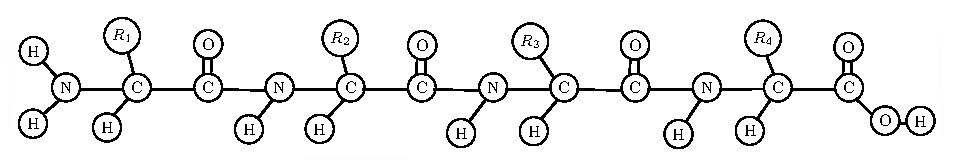
\includegraphics{aa3_1.eps}
}

\textbf{Вторичная структура} задается укладкой цепочки аминокислот в пространственные структуры, \textbf{третичная структура} - расположением этих структур в пространстве в случае, когда белок содержит только одну цепь.

Когда белок состоит из нескольких цепей, говорят о его \textbf{четвертичной структуре}.
\end{frame}

\begin{frame}{Белки и энергия}
С точки зрения химии, разным видам структуры соответствуют разные виды химических связей и электростатических взаимодействий.

Когда мы рассматриваем несколько цепочек в составе одного белка или несколько белков, образующих комплекс, мы говорим о \textbf{белок-белковом взаимодействии}.

\textbf{Интерфейс} такого взаимодействия -- это участки \textbf{поверхности} белков, непосредственно контактирующие между собой.

\end{frame}
\begin{frame}{Белок-белковое взаимодействие - I}
\begin{center}
\resizebox{!}{0.5\textheight}{
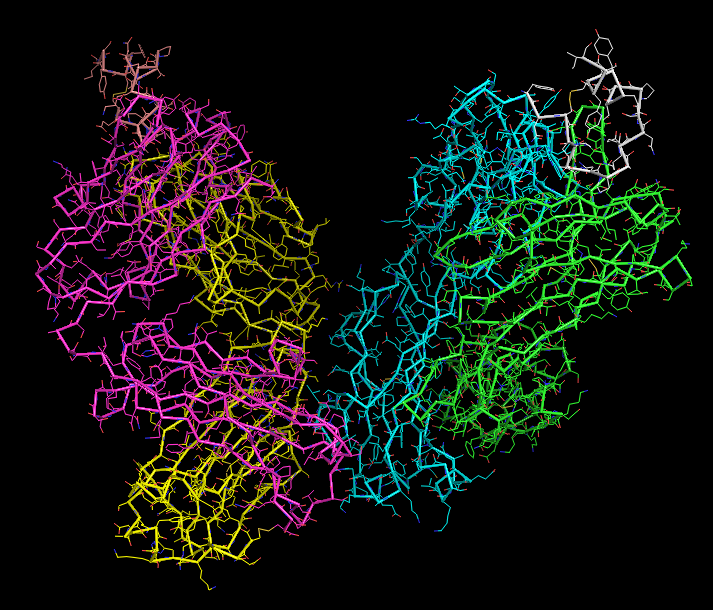
\includegraphics{antibody.png}
}
\end{center}
Рассмотрим белок, имеющий четвертичную структуру.

\textbf{Вопрос}: можно ли изменить что-то в его структуре, чтобы образующие его цепочки были лучше сцеплены между собой?
\end{frame}
\begin{frame}{Белок-белковое взаимодействие - II}
Пусть есть комплекс из двух белков (например, имунноглобулин и эпитоп).

\textbf{Вопрос 1}: можно ли изменить что-то в его структуре, чтобы усилить связь между компонентами комплекса?

\textbf{Вопрос 2}: насколько специфична одна из компонент комплекса?  Можно ли подобрать один из белков так, чтобы комплекс был более устойчивым? Насколько заменяема каждая из компонент?

Ответить нам поможет \textbf{аланиновое сканирование} (аланиновый мутагенез).
\end{frame}

\begin{frame}{Аланиновое сканирование}

Аланиновое сканирование (ала-скан)\footnote{2001, "Combinatorial alanine-scanning" (Morrison K.L., Weiss G.A.).}  - метод для определения аминокислот в составе белка, играющих важную роль в сохранении его функций, стабильности или формы.
\begin{wrapfigure}{RT}{0.3\textwidth}
\resizebox{0.3\textwidth}{!}{
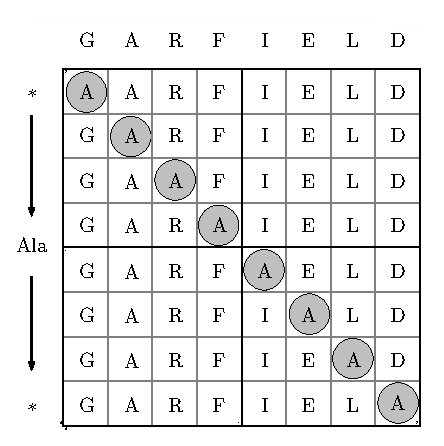
\includegraphics{intro/ala_scan.eps}
}
\end{wrapfigure}

Проблемы ala-scan in vitro/in vivo:
\begin{itemize}
\item Большое пространство поиска.
\item Сложность синтеза библиотек: необходим индивидуальный подход!
\item Высокая стоимость.
\end{itemize}
\end{frame}
\begin{frame}{Энергетически горячие аминокислотные остатки}
Энергетически горячий остаток (ЭГО)\footnote{в англоязычной литературе ,,energy hotspot residue''} -- такая аминокислота в составе одного из компонент белок-белкового комплекса, мутагенез  которой приводит существенному изменению свободной энергии комплекса $\Delta\Delta G$.

Существенным обычно считают изменение, превышающее по модулю 0.5-1 килокалорий на моль.

Цель аланинового сканирования -- найти ЭГО.

Но для больших белков по всем аминокислотам его проводить долго, поэтому производится предварительный отбор аминокислот.
\end{frame}

\begin{frame}{Ala-scan in silico}{Компьютерное моделирование аланинового сканирования. Постановка задачи}
\textbf{На входе}: Пространственная структура белкового комплекса (в формате PDB).

\textbf{На выходе}: ЭГО.

\textbf{Как решить}: 
вычислить потери свободной энергии $\Delta\Delta G$ при замене аминокислотного остатка на аланин для всех аминокислот, выбрать позиции с существенным значением потери (как правило, существенным считают изменение больше 1 килокалории на моль).
\end{frame}

\begin{frame}{Ala-scan in silico}{Компьютерное моделирование аланинового сканирования. Методы}
"Computational alanine scanning of protein-protein interfaces" (Kortemme, et al. - 2004)

"Computational Alanine Scanning Mutagenesis - An Improved Methodological Approach" (I.S. Moreira, et al. - 2006)

Готовые решения используют (на этапе мутагенеза): 
\begin{itemize}
\item решения уравнения Пуассона-Больцмана (MM-PBSA)
\item метод возмущения свободной энергии
\item обобщенный метод Борна
\item метод Монте-Карло
\end{itemize}
Посмотрим, как выбирают области для аланинового сканирования.
\end{frame}
\begin{frame}{Выбор регионов для сканирования I}{Использование отсечки по расстоянию}
\begin{itemize}
\item Аланиновому сканированию подвергаются аминокислоты цепочки, образующей комплекс совместно с другой цепочкой, содержащие атомы, удаленные от каких-либо атомов цепочки, также участвующей в образовании комплекса, на расстояние, не превышающей некоторой фиксированной величины

\item В качестве порогового значения расстояния используются, например, величины 4, 5, 8 A

\item в Rosetta Alascan Protocol используется усложнение: дополнительно рассматриваются аминокислоты, $\beta$-углерод которых после формирования комплекса в шаре определенного фиксированного радиуса содержит существенно больше атомов $\beta$-углерода, чем содержал до этого.
\end{itemize}
%Почему проводят не по всем позициям
%как выбирают
%методы
\end{frame}
\begin{frame}{Эксперимент}
\begin{itemize}
\item Рассмотрим базу данных с информацией о результатах эспериментов по аланиновому сканированию ASEdb.
\item Найдем объекты со ссылкой на Protein Data Bank.
\item Среди всех таких объектов, найдем те, в которых есть аминокислоты, мутация которых приводит к существенному изменению свободной энергии комплекса ($\geq 1$ ккал/моль)
\item Посмотрим, всегда ли они удалены от интерфейса в пределах стандартно используемой отсечки (в качестве примера возьмем расстояние, не превышающее 8 \AA{}).
\end{itemize}
\end{frame}
\begin{frame}{Результаты эксперимента}
Комплекс человеческого гормона роста и рецептора человеческого гормона роста\footnote{идентификатор структуры в Protein Data Bank -- 3hhr}
%1. картинка с примером
\begin{center}
\resizebox{!}{0.5\textheight}{
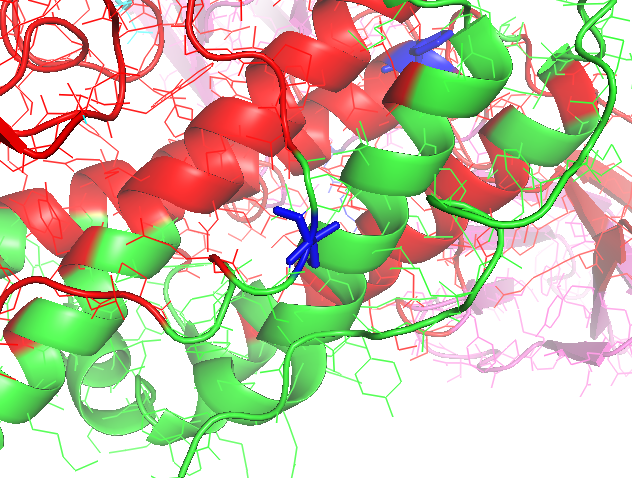
\includegraphics{intro/image7.png}
}
\end{center}
\end{frame}

\begin{frame}{Выбор регионов для сканирования II}{Поиск по гомологии}

ASEdb: 76/101 корректных записей о белках, из них много 3hhr.

Еще одна замечательная база данных:
\begin{center}
\resizebox{!}{0.6\textheight}{
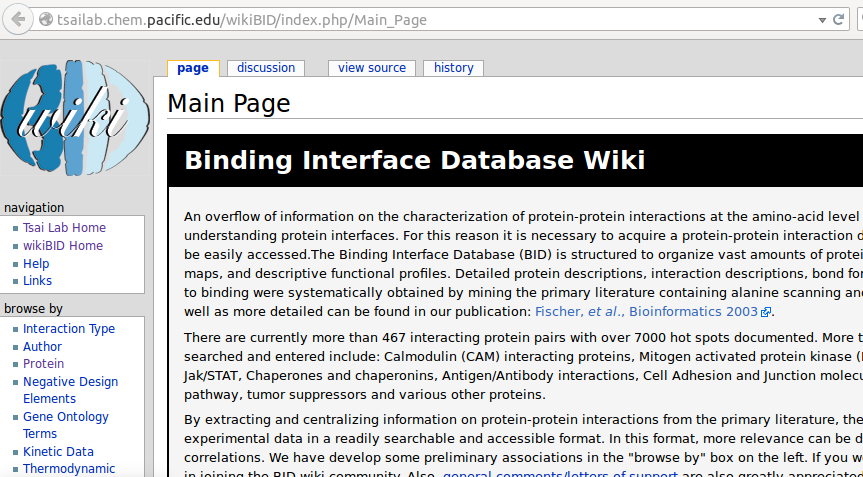
\includegraphics{exp2.png}
}
\end{center}
\end{frame}

\begin{frame}{Выбор регионов для сканирования II}{Выводы. Основная задача.}

Выводы: эффективного и универсального метода способа найти ЭГО -- не придумали.

Будем решать эту задачу. Для этого попробуем по полученной картинке понять, что еще необходимо учесть:
%1. картинка с примером
\begin{center}
\resizebox{!}{0.5\textheight}{
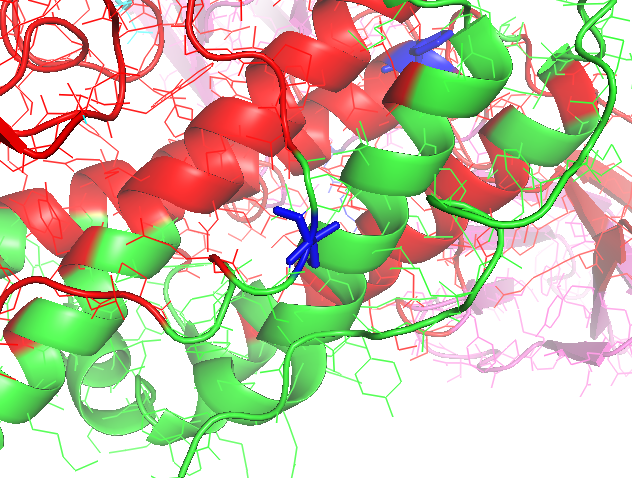
\includegraphics{intro/image7.png}
}
\end{center}
\end{frame}

\begin{frame}{Как будем выбирать регионы для сканирования}
\begin{itemize}
\item разумно начинать с области интерфейса белок-белкового взаимодействия, затем расширять ее.
\item при мутации не гидрофобные аминокислоты могут стать гидрофобными и оказаться значимыми, поэтому в первую очередь можно расширить область на такие аминокислоты, находящиеся на границе интерфейса.
\item поскольку при выборе интерфейса с отсечкой по расстоянию в интерфейсе могут появляться дыры, будем их заполнять. Для этого будем искать поверхностные карманы (углубления в поверхности белка в границах интерфейса).
\item Из всех вторичных структур на поведение белка больше всего влияют петли. Добавим в интерфейс все аминокислоты, содержащиеся в петлях, которые частично уже попали в область рассмотрения.
\end{itemize}
\end{frame}


\begin{frame}{Алгоритм поиска протяженных регионов,}{ потенциально содержащих ,,энергетически горячие точки''}
Включим в состав множества протяженных регионов, содержащих ,,энергетически горячие аминокислотные остатки'', следующее:
\begin{itemize}
\item аминокислоты, образующие ,,интерфейс'' взаимодействия с парной цепочкой или белком (с использованием отсечки по расстоянию от второй цепочки)
\item аминокислоты, образующие поверхность ,,карманов'', находящихся в области взаимодействия пары белков
\item не-гидрофобные аминокислоты, являющиеся соседними по отношению к аминокислотам, образующим интерфейс
\item если интерфейс взаимодействия образован петлями, то добавим все аминокислоты, образующие петли 
\end{itemize}


\end{frame}
\begin{frame}{,,Интерфейс''}
\begin{itemize}
\item определяем множество треугольников выпуклой оболочки, для которых хотя бы одна вершина удалена от центров атомов второй цепочки не больше, чем на выбранное значение отсечки
\item Далее расширяем интерфейс
\begin{itemize}
\item шаг 1: добавляем к интерфейсу все треугольники выпуклой оболочки, содержащие атомы аминокислот, которые уже туда попали
\item шаг 2: продлеваем регион до границы гидрофобности
\item шаг 3: продлеваем регион за границы гидрофобности на 1 аминокислоту.
\end{itemize}
\end{itemize}


В результате у нас есть одна или нескольких протяженных связных областей выпуклой оболочки, по которым можно восстановить аминокислоты.
\end{frame}


\section{Поиск регионов}
\begin{frame}{Триангуляция Делоне}
\begin{itemize}
\item Рассматриваем одновременно 2 цепочки, образующие белковый комплекс.
\item Начнем с построения выпуклой оболочки и триангуляции Делоне для каждой из них, будем искать протяженные регионы с энергетически горячими аминокислотными остатками  на одной из них. Строить будем по центрам атомов, формирующих аминокислоты цепочки.
\item Выберем все треугольники выпуклой оболочки, в которых хотя бы одна вершина удалена от некоторых атомов второй цепочки не далее, чем на выбранное (фиксированное) значение отсечки.
\end{itemize}
\end{frame}

\begin{frame}{Построение графа по триангуляции Делоне}
\begin{center}
\resizebox{!}{0.5\textheight}{
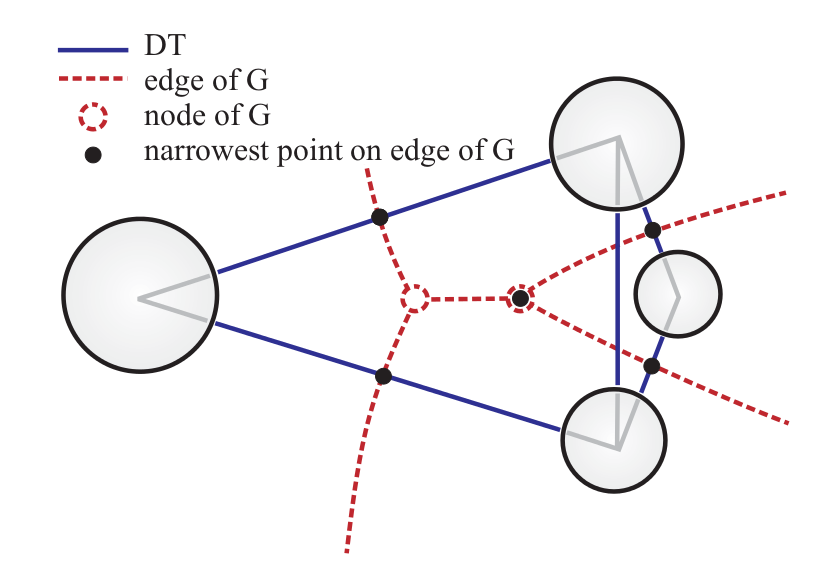
\includegraphics{algorithm/image4_caver.png}
}

[Computation of tunnels in protein molecules using
Delaunay triangulation, P.Medek, et al., 2007]
\end{center}

Используем модифицированный алгоритм Дейкстры, аналогично упомянутому в оригинальной работе.
\end{frame}

\begin{frame}{Петли}

Перед добавлением петель треугольники триангуляции преобразуются в фрагменты последовательности аминокислот, продлеваем их, используя информацию о вторичной структуре.

\end{frame}
\section{Аланиновое сканирование}

\begin{frame}{Ala-scan in silico с фильтрацией данных}{Реализация}
\textbf{Полученный алгоритм аланинового сканирования} основан на Rosetta alascan protocol и образован следующей последовательностью действий:
\begin{itemize}
\item читаем 2 цепочки атомов из PDB,
\item выбираем аминокислоты одной из цепочек с помощью приведенного выше алгоритма поиска,
\item для этих аминокислот пробуем провести мутагенез с использованием метода Монте-Карло выводим те, изменение которых привело к существенным изменениям свободной энергии системы.
\end{itemize}
\end{frame}

\begin{frame}{Результаты}
\begin{itemize}
\item Получен скрипт, который итеративно формирует протяженные регионы, содержащие ЭГО (в процессе тестирования), и который может использоваться в модифицированном rosetta ala-scan protocol для поиска аминокислотных последовательностей.
\item Планируется: переделать в плагин к PyMol, добавить промежуточный вывод аминокислот для визуального воспроизведения (в виде mesh-объекта)
\item Предоположительно, в алгоритм можно добавить поиск по гомологии (на стадии идеи)
\end{itemize}
\end{frame}

\section{Результаты}
%здесь должны быть скриншоты из PyMol,
%на которых видно выделение областей в отдельный mesh

\begin{frame}{}
Вопросы?
\end{frame}
\begin{frame}


\begin{center}
\resizebox{\textheight}{!}{
\ttfamily
\footnotesize
\aapicture
}
\end{center}

\end{frame}

\end{document}

